\documentclass[12pt]{amsart}
\usepackage{preamble}
\usepackage{rotating}
\DeclareMathOperator{\stab}{\mathrm{stab}}

\begin{document}
\begin{center}
    \textsc{Math 601. HW A\\ Ian Jorquera}
\end{center}
\vspace{1em}
\begin{itemize} %
    \item[(1)]
    First recall that any $\mathfrak{sl}_3$ crystal has a unique highest weight word 
    which is ballot. When looking that crystal with weight $(3,3,0)$ we can consider the 
    ballot word $222111$ and build the crystal as to be the following

    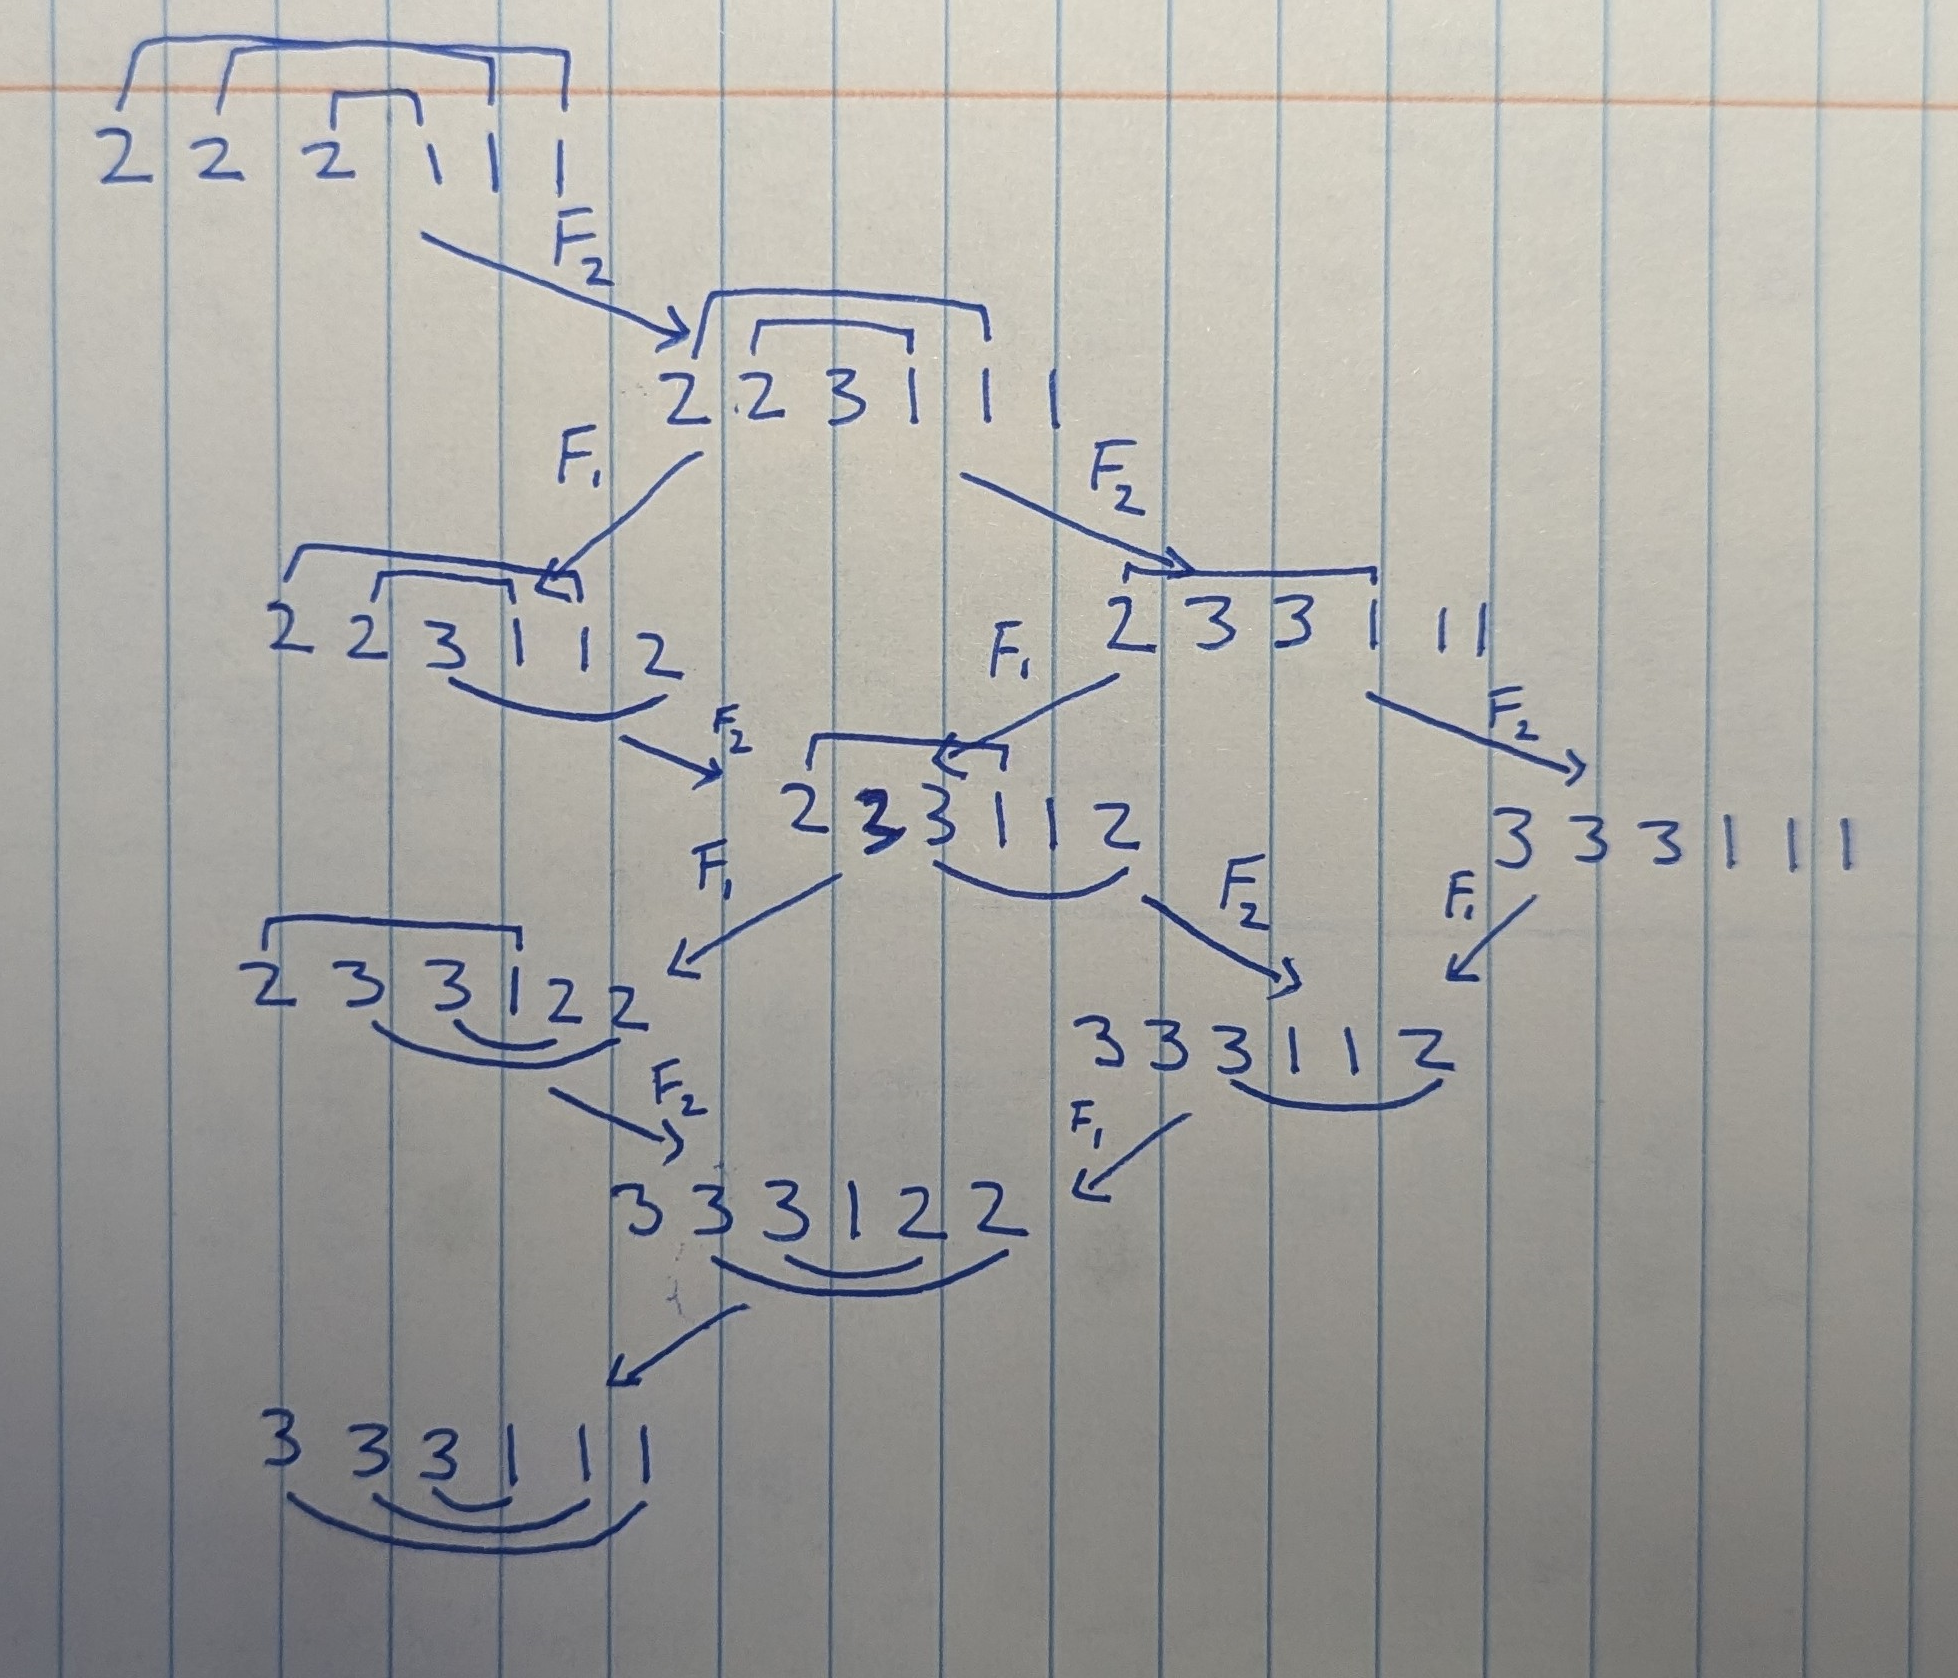
\includegraphics[scale=.16]{hwb-1.png}

    \item[(2)]
    Recall that the hyperoctahedral group are the signed permutations. We can consider it to be 
    the permutations in $S_{\{\pm 1,\dots,\pm n\}}$ such that each permutation satisfies 
    $w(-i)=-w(i)$. Now consider a permutation $w$ and elements $a_1\in [\pm n]$ that is 
    not fixed by the permutation. We may consider the maximal sequence $a_1,a_2,\dots,a_n$
    of entries such that absolute values $|a_j|$ are distinct for all $j$.
    Notice that this means there would have to be the negative of this sequence
    $-a_1,-a_2,\dots,-a_n$ meaning $-a_i\mapsto -a_j$ whenever $a_i\mapsto a_j$. 
    There are two cases first $a_n\mapsto a_1$ and so $-a_n\mapsto -a_1$ which gives use the 
    two cycles $(a_1,a_2,\dots,a_n)(-a_1,-a_2,\dots,-a_n)$. The second case is when 
    $a_n\mapsto -a_\ell$ for some $a_\ell$ already in the sequence. Because this is a permutation
    it must be the case that $a_n\mapsto -a_1$ create the cycle $(a_1,a_2,\dots,a_n,-a_1,-a_2,\dots,-a_n)$.\\

    \item[(3)]
    We will use the definition $\mathfrak{s0}_{2n+1}=\{X\in \C^{2n+1\times 2n+1}: X^tS+SX=0\}$ where 
    \[S=\begin{bmatrix}[c|cc]
        1 &0 &0\\
        \hline
        0 &0 &I_n\\
        0 &I_n& 0
    \end{bmatrix}\]
    Notice that because $S$ is a permutation matrix $S^{-1}=S^t$ and because 
    $S$ is symmetric, $S^{-1}=S^t=S$. So we can rewrite the defining equation as $X^t=-SXS$.
    Now let $X_1,X_2,X_3,X_4\in \C^{n\times n}$, and $y_1,y_2,y_3,y_4\in \C^n$ then 
    \[X=\begin{bmatrix}[c|ccc|ccc]
        0 &&y_1^t&&&y_2^t&\\
        \hline
        &&&&&&\\
        y_3&&X_1&&&X_2&\\
        &&&&&&\\
        \hline
        &&&&&&\\
        y_3&&X_1&&&X_2&\\
        &&&&&&\\
    \end{bmatrix} X^t=\begin{bmatrix}[c|ccc|ccc]
        0 &&y_3^t&&&y_4^t&\\
        \hline
        &&&&&&\\
        y_1&&X_1^t&&&X_3^t&\\
        &&&&&&\\
        \hline
        &&&&&&\\
        y_2&&X_2^t&&&X_4^t&\\
        &&&&&&\\
    \end{bmatrix} SXS=\begin{bmatrix}[c|ccc|ccc]
        0 &&-y_2^t&&&-y_1^t&\\
        \hline
        &&&&&&\\
        -y_4&&-X_4&&&-X_3&\\
        &&&&&&\\
        \hline
        &&&&&&\\
        -y_3&&-X_2&&&-X_1&\\
        &&&&&&\\
    \end{bmatrix}\]
    Giving us $y_1=-y_4$, $y_2=-y_3$, $X_1^t=-X_4$, $X_2^t=-X_2$, $X_3^t=-X_3$ which tells 
    us about the redundant basis elements $\mathfrak{s0}_{2n+1}$. This gives us 
    \[\left\{\begin{bmatrix}[c|ccc|ccc]
        0 &&y_1^t&&&y_2^t&\\
        \hline
        &&&&&&\\
        -y_2&&X_1&&&X_2&\\
        &&&&&&\\
        \hline
        &&&&&&\\
        -y_1&&X_3&&&-X_1^t&\\
        &&&&&&\\
    \end{bmatrix} \Bigg|\; y_1,y_2\in \C^n, X_1,X_2,X_3\in \C^{n\times n}, X_2^t=-X_2, X_3^t=-X_3 \right\}\]
    This means a basis for $\mathfrak{so}_{2n+1}$ would be the union of the sets
    \begin{equation*}
        \begin{split}
        \{ E_{1(j+1)}-E_{(n+j+1)1}, E_{1(n+j+1)}-E_{(j+1)1} |  1\leq j\leq n\},\\ % for the ys
        \{E_{(i+1)(j+1)}-E_{(n+j+1)(n+i+1)} | 1\leq i, j\leq n\},\\ % for X_1, X_4
        \{E_{(i+1)(n+j+1)}-E_{(j+1)(n+i+1)}, E_{(n+i+1)(j+1)}-E_{(n+j+1)(i+1)} | 1\leq i \leq j\leq n 
        \}
        \end{split}
    \end{equation*}
    Where the first set comes from the $y$'s, the second from $X_1$ and the third from $X_2$ and $X_3$.
    With this construction the Cartan subalgebra are the diagonal matrices, which
    have a basis of $\{E_{(j+1)(j+1)}-E_{(n+j+1)(n+j+1)}|2\leq j\leq n+1\}$

    Define $L_j$ to be the project of the $(j+1,j+1)$ entry of any such diagonal entry.
    To determine the roots we can see how the Cartan subalgebra acts on the basis given above.
    Where we can determine the roots to be the union of the sets 
    $\{\pm L_j |1\leq j\leq \}$, $\{\pm (L_i-L_j) |1\leq j\leq \}$ and 
    $\{\pm (L_i+L_j) |1\leq j\leq \}$ each coming from the corresponding set from the basis.
    This is exactly the type B root system.\\

    \item[(4)]
    This follows from HW 6 problem 3. Where we found that the dimension of the adjoint representation of 
    $\mathfrak{so}_{2n+1}$ was $2n^2+n$ meaning $\dim(\mathfrak{so}_{7})=21$\\
    
    \item[(5)]
    let $\{\phi_1,\phi_2,\phi_3,\phi_4,\phi_5\}$ be the vectors corresponding to the $5$th 
    roots of unity, of unit norm. Notice that $\ip{\phi_1,\phi_2}=\cos(2\pi/5)$ which is not half an integer!
    This means the $5$th roots of unit can not be a root system as the do not satisfy the second condition
    corresponding to the angles between any two roots.\\


    \item[(6)] 
    Here we can do the evacuation and then do it again
    
    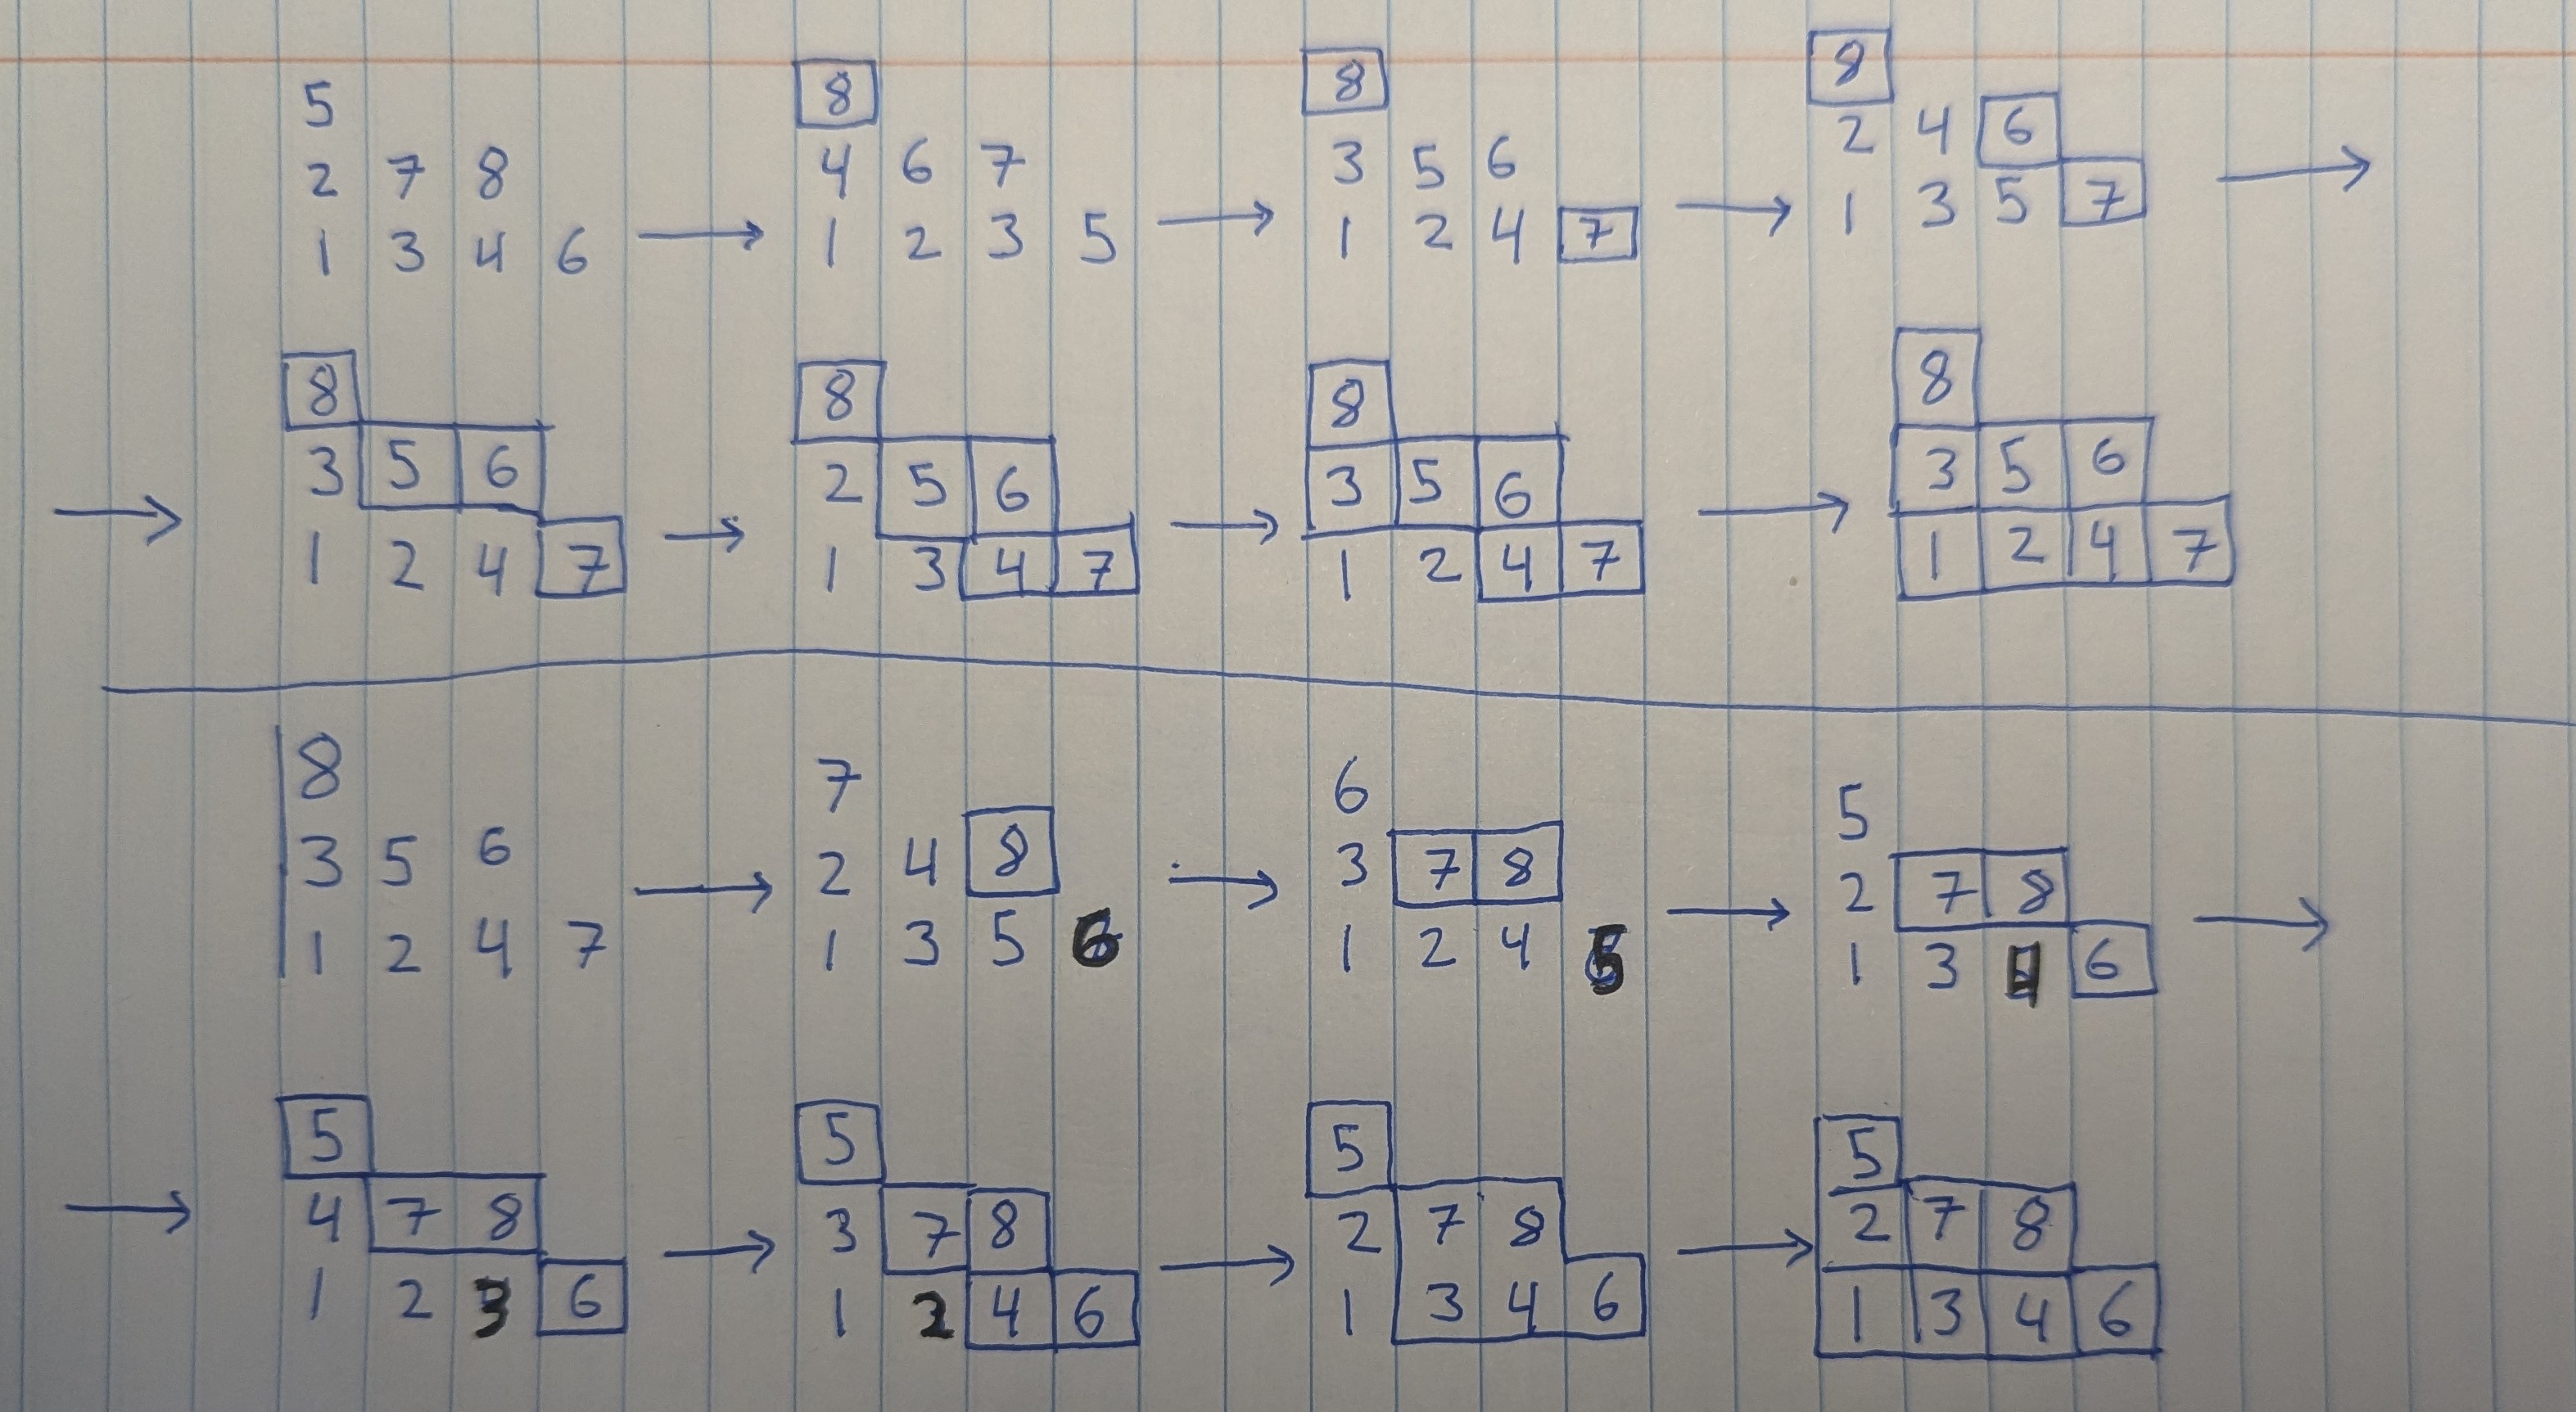
\includegraphics[scale=.1]{hwb-2.jpg}


    \item[(7)]
    $\tilde{H}_{(2,1,1)}(x;q)=s_{(4)}+(q^1+q^2)s_{(3,1)}+q^3s_{(2,1,1)}$
    \item[(8)]
    Consider the word $w=w_1\dots w_n$ with content $\mu$ where $\mu$ is a partition with $w_1\neq 1$
    Because computing cocharge for partition content takes place in rounds, each time 
    picking the first occurrence of every number, 
    moving $w_1$ to the end of the word would not affect the round in which it is labeled. This 
    means we can consider only that particular round, 
    and we may assume that $w$ is a partition in list notation.

    Consider a partition in list notation $w=w_1\dots w_n$.
    Notice that if $w_1\neq 1$ then there must exist a $w_1-1$ somewhere in the suffix
    $w_2\dots w_n$, which we will assume occurs in position $\ell$. In the process of 
    computing cocharge, we would annotate $w_\ell$ with $a$ and the then ${w_1}$ with an $a+1$.
    Continuing the process we would then annotate some $w_1+1$ with a $a+1$ again, and so on.
    But then notice for the word $w'=w_2\dots w_n w_1$ we would again annotate $w_\ell$ with an $a$ as 
    the $w_1$ moving wont affect it, as it is a larger number. Then in this case $w_1$ would be annotated
    with an $a$ and continuing the process we would then annotate some $w_1+1$ with a $a+1$. This 
    meas the only annotation that changes is the annotation on the $w_1$ which reduced by $1$.
    So $cc(w')=cc(w)-1$.\\
    \item[(9)]
    Consider the word $123$ which has $cc(123)=0$ but $cc(231)=1\neq -1$
\end{itemize}

\end{document}

